\input ../SlidePreamble
\input ../preamble


\begin{document}

{\Huge

  \centerline{\bf TTIC 31230, Fundamentals of Deep Learning}
  \bigskip
  \centerline{David McAllester, Winter 2019}
  \vfill
  \centerline{\bf Generative Adversarial Networks (GANs)}
  \vfill
\vfill
\vfill

\slide{Representing a Distribution with a Generator}
\centerline{$z\sim {\cal N}(0,I)$ \hspace{7em} $y\sim P_\Phi$}
\centerline{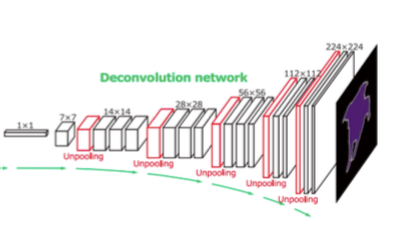
\includegraphics[width=6in]{../images/halfdeconv}}


\slidetwo{Generative Adversarial Nets}{Goodfellow et al., June 2014}

Let ${\color{red} \pop \uplus P_\Phi}$ be the distribution defined flipping an unbiased coin and, if heads, returning {\color{red} $(1,y)$} with
{\color{red} $y \sim \pop$} and, if tails, returning {\color{red} $(-1,y)$} with {\color{red} $y \sim P_\Phi$}.

{\color{red} $$\Phi^* = \argmax_\Phi \min_\Psi \;E_{(i,y) \sim (\pop \uplus P_\Phi)} - \ln P_\Psi(i|y)$$}
\centerline{/\hspace{2.5em} $\backslash$ \hspace{9.5em}~}
\centerline{Generator \hspace{2em}Discriminator \hspace{8em}~}

\vfill
Assuming Universality: {\color{red} $P_{\Phi^*} = \pop$}

\slidetwo{Generative Adversarial Nets}{Goodfellow et al., June 2014}
\centerline{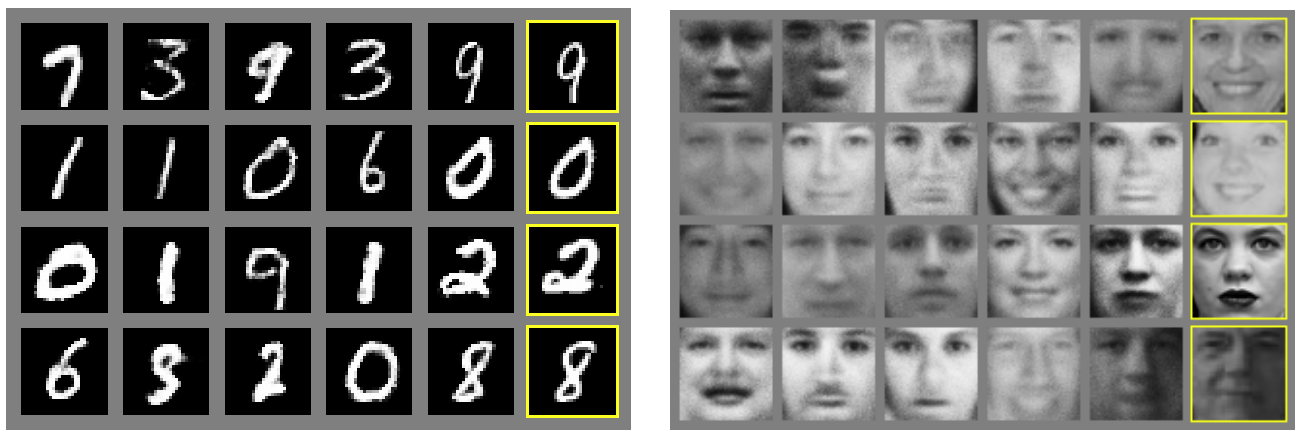
\includegraphics[width = 9in]{../images/GAN2014}}

\slidetwo{Unsupervised Representation Learning ... (DC GANS)}
{Radford et al., Nov. 2015}

\centerline{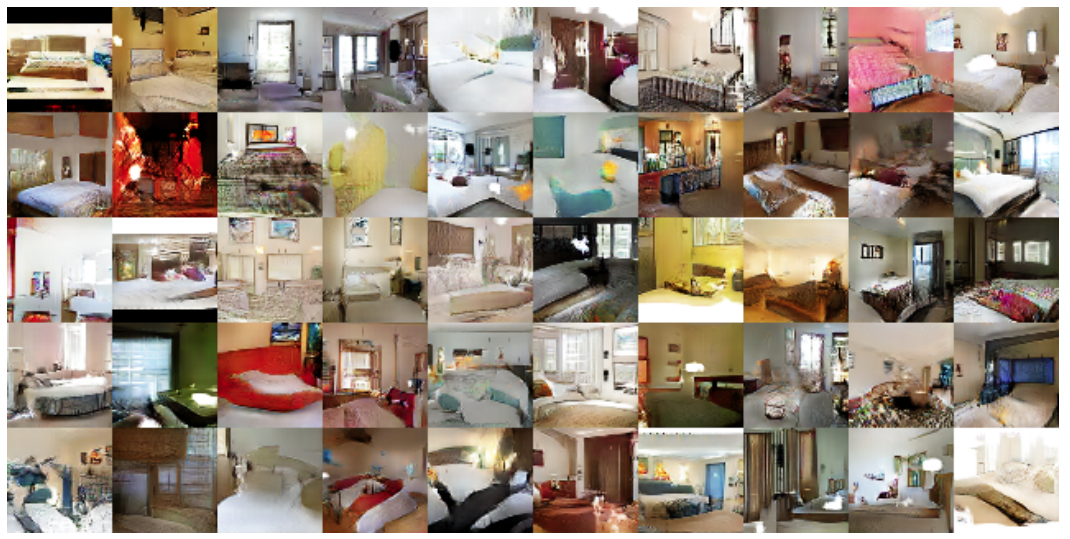
\includegraphics[width = 9in]{../images/GANDCa}}

\slidetwo{Unsupervised Representation Learning ... (DC GANS)}
{Radford et al., Nov. 2015}

\centerline{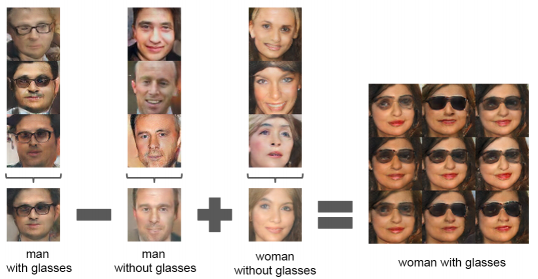
\includegraphics[width = 9in]{../images/ImageFeatures}}

\slide{Interpolated Faces}

[Ayan Chakrabarti]

\centerline{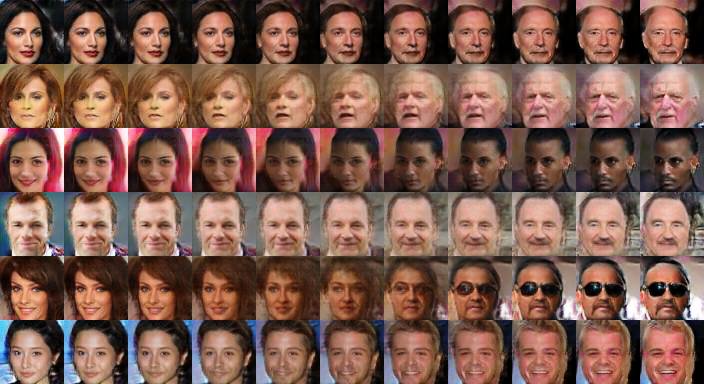
\includegraphics[height = 4.5in]{../images/interp}}

\slide{Early GANs on ImageNet}

\centerline{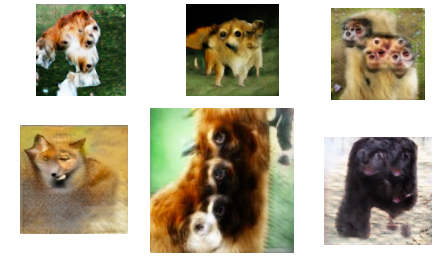
\includegraphics[height = 4.5in]{../images/BadGAN}}


\slide{Conditional GANs}

All distribution modeling methods apply to conditional distributions.

$${\color{red} \Phi^* = \argmax_\Phi \; \min_\Psi \;\expectsub{i,x,y \sim (\mathrm{Pop}\; \uplus \;\mathrm{Pop}(x)P_\Phi(y|x))}
  {-\ln P_\Psi(i|x,y)}}$$

If $x$ is never repeated we can replace $P_\Phi(y|x)$ by a deterministic function $\hat{y}_\Phi(x)$.


$${\color{red} \Phi^* = \argmax_\Phi \; \min_\Psi \;\expectsub{i,x,y \sim (\mathrm{Pop}\; \uplus \;(\mathrm{Pop}(x);\hat{y}(x)))}
  {-\ln P_\Psi(i|x,y)}}$$


\slide{Discrimination Loss can Augment Distortion Loss}

$${\color{red} \Phi^* = \argmin_\Phi\; \expectsub{x,y \sim \mathrm{Pop}} \mathrm{Dist}(y,\hat{y}_\Phi(x))}$$

This is the fundamental equation if {\color{red} $\mathrm{Dist}(y,\hat{y}_\Phi(x)) = -\ln P_\Phi(y|x)$}.

\vfill
$$\Phi^* = \argmin_\Phi\;{\cal L}_{\mathrm{Dis{\color{red}t}}}(\Phi) + \lambda{\cal L}_{\mathrm{Dis{\color{red}c}}}(\Phi)$$

$${\cal L}_{\mathrm{Dis{\color{red}t}}}(\Phi) =  \expectsub{x,y \sim \mathrm{Pop}} \mathrm{Dis{\color{red}t}}(y,\hat{y}_{\Phi}(x))$$

$${\cal L}_{\mathrm{Dis{\color{red}c}}}(\Phi) = \max_\Psi \;\expectsub{i,x,y \sim (\mathrm{Pop}\; \uplus \;(\mathrm{Pop}(x);\hat{y}_\Phi(x)))}
  {\ln P_\Psi(i|x,y)}$$

\slidetwo{Image-to-Image Translation (Pix2Pix)}
{Isola et al., Nov. 2016}

We assume a corpus of ``image translation pairs'' such as images paired with semantic segmentations.

\centerline{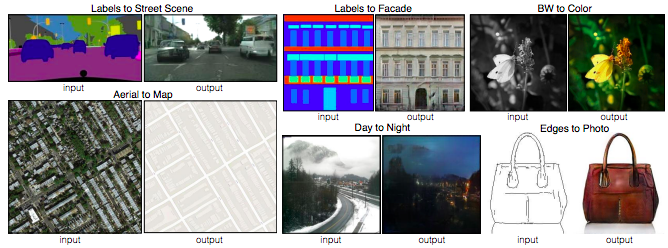
\includegraphics[width = 8.0in]{../images/cGAN0}}

\slidetwo{Image-to-Image Translation (Pix2Pix)}
{Isola et al., Nov. 2016}

\centerline{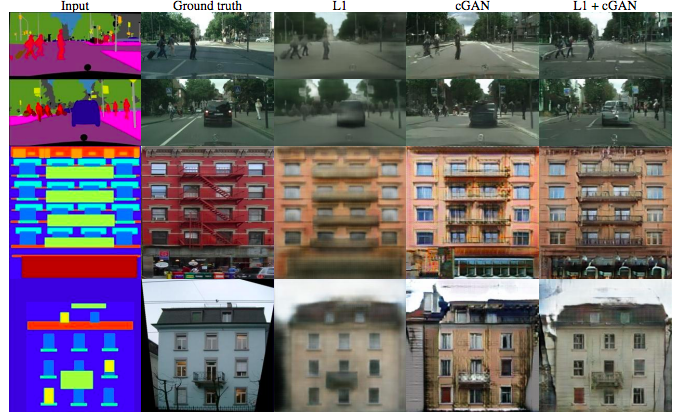
\includegraphics[height = 4.5in]{../images/cGAN1}}

\slide{Arial Photo to Map and Back}

\centerline{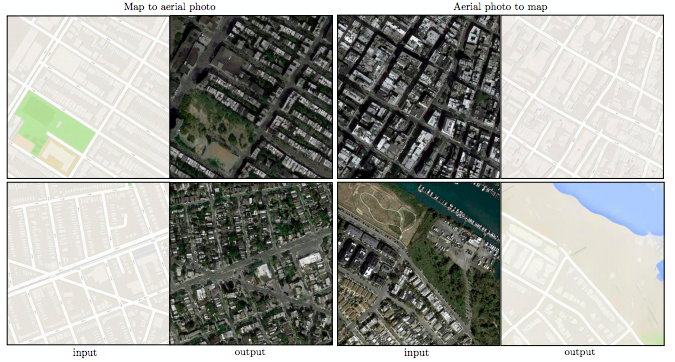
\includegraphics[width = 8.0in]{../images/cGAN2}}

\slide{Colorization}

\centerline{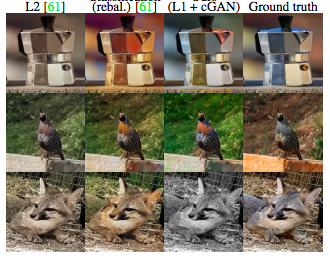
\includegraphics[width = 6.0in]{../images/cGAN3}}

\slide{Semantic Segmentation}

\centerline{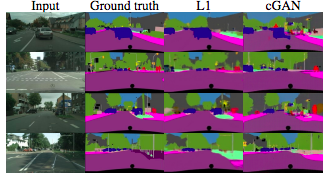
\includegraphics[width = 8.0in]{../images/cGAN4}}

\slidetwo{Unpaired Image-to-Image Translation (Cycle GANs)}{Zhu et al., March 2017}

We have two corpora of images, say images of zebras and unrelated images of horses, or photographs and unrelated paintings by Monet.

\vfill
We want to construct translations between the two classes.

\centerline{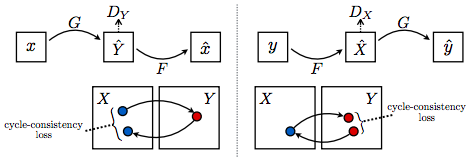
\includegraphics[width = 8.0in]{../images/Cycle2}}

\slide{Cycle Gans}

\centerline{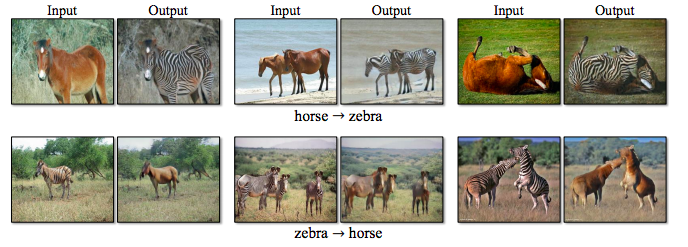
\includegraphics[width = 11.0in]{../images/Cycle3}}

\slide{Cycle Gans}

\centerline{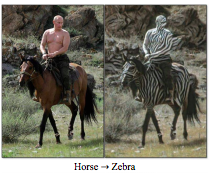
\includegraphics[width = 6.0in]{../images/Cycle4}}

\slidetwo{Unsupervised Machine Translation (UMT)}
         {Lample et al, Oct. 2017, also Artetxe et al., Oct. 2017}

\centerline{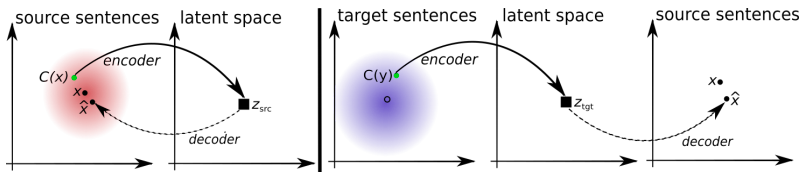
\includegraphics[width = 10.0in]{../images/Cycle5}}

\slide{Text to Speech (Saito et al. Sept. 2017)}

\centerline{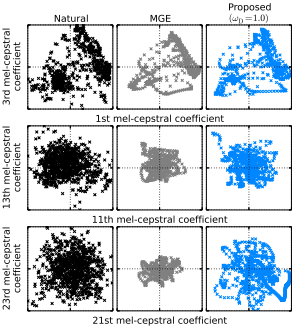
\includegraphics[width = 3.0in]{../images/Txt2spchGAN}}

\vfill
Minimum Generation Error (MGE) uses {\color{red} perceptual distortion} ---
a distance between the feature vector of the generated sound wave and the
feature vector of the original.

\vfill
{\color{red}Perceptual Naturalness} can be enforced by a discriminator.

\slidetwo{Adversarial Discriminative Domain Adaptation}{Tzeng et al. Feb. 2017}

\centerline{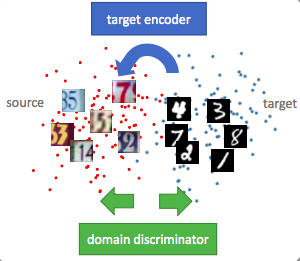
\includegraphics[width = 4.0in]{../images/AdvDomainAdapt}}

A GAN is used to map target images to the source feature distribution.

\slidetwo{Progressive Growing of GANs}{Karras et al., Oct. 2017}
\centerline{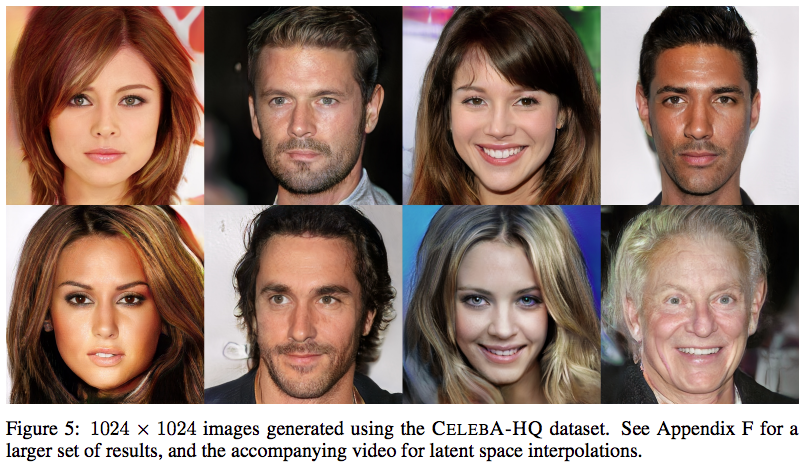
\includegraphics[height = 4.5in]{../images/GANproga}}

\slidetwo{Progressive Growing of GANs}{Karras et al., Oct. 2017}
\centerline{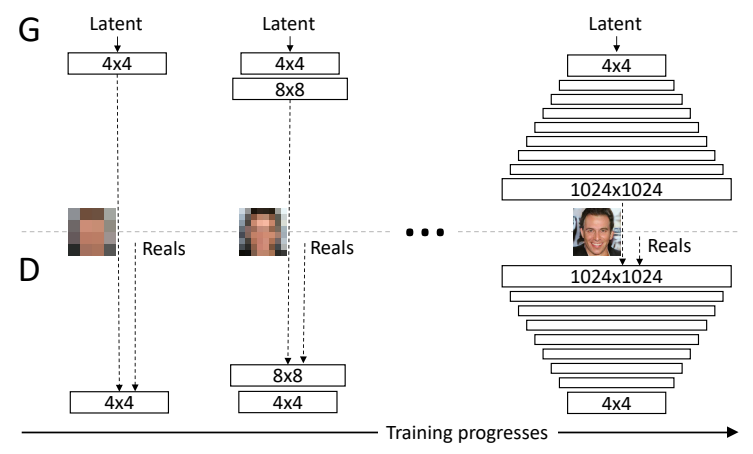
\includegraphics[height = 4.5in]{../images/GANprogb}}

\slidetwo{Progressive Growing of GANs}{Karras et al., Oct. 2017}
\centerline{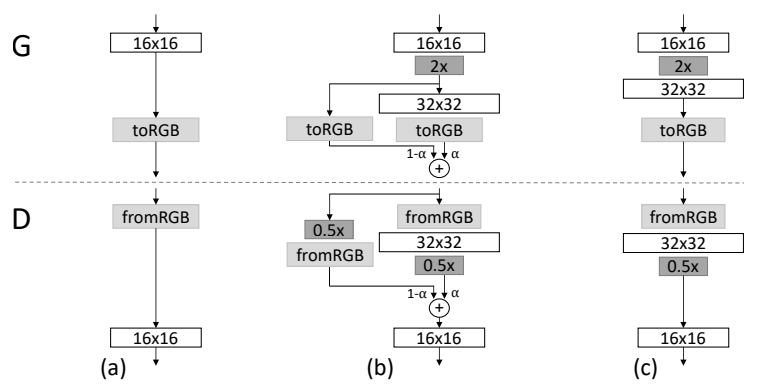
\includegraphics[height = 4.5in]{../images/GANprogc}}

\slidetwo{Large Scale Gan Training}{Brock et al., Sept. 2018}
\centerline{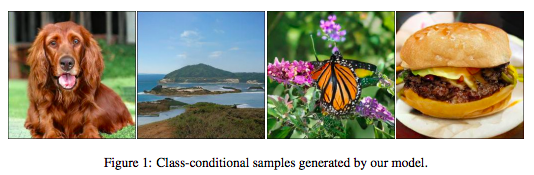
\includegraphics[width = 9in]{../images/GANclass}}

\vfill
This is a conditional GAN conditioned on the imagenet class label.

\vfill
This generates 512 X 512 images without using progressive training.

\slide{Issues}

\centerline{Jensen-Shannon Divergence}

\vfill
\centerline{Vanishing Gradients}

\vfill
\centerline{Unstable Training}

\vfill
\centerline{Mode Collapse}

\vfill
\centerline{Measuring Perfomance}



\slide{Discrimination: Jensen-Shannon Divergence}

Assuming Universality:
\begin{eqnarray*}
& & {\color{red} E_{(i,y) \sim (\pop\uplus Q)}\;-\ln P_{\Phi^*}(i|y)} \\
\\
& = & E_{(i,y) \sim (\pop\uplus Q)}\;-\ln P(i|y) \\
\\
& = & \frac{1}{2}E_{y \sim \pop} -\ln\;\frac{\pop(y)}{\pop(y) + Q(y)}+ \frac{1}{2} E_{y \sim Q}\; -\ln\;\frac{Q(y)}{\pop(y) + Q(y)} \\
\\
\\
& = & {\color{red} (\ln 2) - \frac{1}{2} \left(\;KL\left(\pop,\frac{\pop+Q}{2}\right),\;KL\left(Q,\frac{\pop+Q}{2}\right)\right)}
\end{eqnarray*}

\slide{Discrimination: Jensen-Shannon Divergence}

\begin{eqnarray*}
& & {\color{red} E_{(i,y) \sim (\pop\uplus Q)}\;-\ln P_{\Psi^*}(i|y)} \\
\\
& = & (\ln 2) - \frac{1}{2} \left(\;KL\left(\pop,\frac{\pop+Q}{2}\right),\;KL\left(Q,\frac{\pop+Q}{2}\right)\right) \\
\\
& = & (\ln 2) + JSD(\pop,Q) \\
\\
\Phi^* & = & \argmin_\Phi \; JSD(\pop,P_\Phi)
\end{eqnarray*}

{\color{red} $$0 \leq JSD(P,Q) \leq \ln 2$$}


\slidetwo{Converting to Cross Entropy}{Goodfellow, 2014}

In Goodfellow's original paper he expressed a preference for cross entropy loss (the fundamental equation) over Jensen-Shannon loss.

$${\color{red} \Phi^* = \argmin_\Phi\;JSD(\pop,P_\Phi)}$$

\centerline{vs.}
\vspace{-2ex}
$${\color{red} \Phi^* = \argmin_\Phi\;H(\pop,P_\Phi)}$$

{\color{red}
$$\begin{array}{lrcl}
\mathrm{GAN:} & \Phi^* & = & \argmin_\Phi\;JSD(P_\Phi,\pop) \\
\\
\mathrm{GAN':} & \Phi^* & = & \argmin_\Phi H(\pop, P_\Phi) \\
\\
\mathrm{contrastiveGAN:} & \Phi^* & = & \argmin_\Phi KL(P_\Phi,\pop)
\end{array}$$
}

\vfill
He presented a modification to the GAN adversarial objective that yields cross-entropy loss rather than Jensen-Shanon loss.

\slidetwo{Converting to Cross Entropy}{Goodfellow, 2014}

{\color{red} $$\Psi^*(\Phi) = \argmin_\Psi \;\expectsub{(i,y) \sim (\mathrm{Pop}\; \uplus \;P_\Phi)}{- \ln P_\Psi(i|y)}$$}

\vfill
$$\mbox{Assume:}\;\;\; P_{\Psi^*}(1|y) = \frac{\mathrm{Pop}(y)}{\mathrm{Pop}(y) + P_\Phi(y)}$$

\vfill
\begin{eqnarray*}
  \mbox{Define:}\;\;\; {\color{red} f_{\Psi^*}(y)} & \doteq & \frac{P_{\Psi^*}(1|y)}{P_{\Psi^*}(-1|y)} \\
\\
& = & {\color{red} \frac{\mathrm{Pop}(y)}{P_\Phi(y)}}
\end{eqnarray*}

\slide{Converting to Cross Entropy}

{\huge
\begin{eqnarray*}
 {\color{red} \Phi^*}& = & {\color{red} \argmax_\Phi\;E_{y \sim \pop} \;f_{\Psi^*}(y)} \\
 \\
 {\color{red} \nabla_\Phi \; E_{y \sim P_\Phi}\;  f_{\Psi^*}(y)}  & = & \nabla _\Phi \sum_y\; P_\Phi(y) f_{\Psi^*}(y) \\
  \\
  & = & \sum_y \; P_\Phi(y) f_{\Psi^*}(y) \nabla_\Phi \ln P_\Phi(y) \\
  \\
  & = & \sum_y \;\mathrm{Pop}(y) \nabla_\Phi \ln P_\Phi(y) \\
  \\
  & = & E_{y \sim \mathrm{Pop}} \; \nabla_\Phi \ln P_\Phi(y) \\
  \\
  & = & {\color{red} \nabla_\Phi \; E_{y \sim \mathrm{Pop}} \;\ln P_\Phi(y)}
\end{eqnarray*}
}

\slide{Vanishing Gradients}

The discriminator typically ``wins''.

\vfill
The log loss goes to zero (becomes exponentially small) and there is no gradient to guide the generator.

\vfill
In this case the learning stops and the generator is blocked from minimizing $\mathrm{JSD}(\mathrm{Pop},P_\Phi)$.

\slide{A Heuristic Fix}

We continue to use

$$\Psi^*(\Phi) = \argmin_\Psi \;\expectsub{(y,s) \sim (\mathrm{Pop}\; \uplus \;P_\Phi)}{- \ln P_\Psi(s|y)}$$

\vfill
But switch the optimization for $\Phi$ from
$$\Phi^* = \argmax_\Phi E_{y \sim P_\Phi}\; - \ln P_\Psi(-1|y)$$

to
$$\Phi^* = \argmin_\Phi E_{y \sim P_\Phi}\;- \ln P_\Psi(1|y)$$

\vfill
It can be shown that $- \ln P_\Psi(1|y)$ is essentially the margin of the binary classifier $\Psi$.


\slide{Mode Collapse a.k.a Mode Dropping}

The generator distribution drops portions of the population.

\centerline{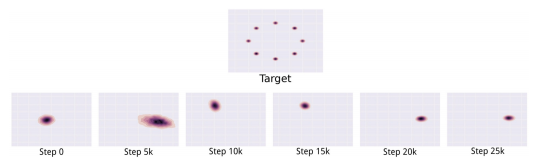
\includegraphics[width=9in]{../images/Unstable1}}

\slide{Unstable Training}

Joint SGD is not the same as nested max-min.

\vfill
Consider
$${\color{red} \max_x \; \min_y\; xy}$$

\vfill
A Nash equilibrium is $x= y = 0$.

\vfill
Simultaneous gradient flow yields a circle.

\slide{Mode Collapse a.k.a Mode Dropping}

The generator distribution drops portions of the population.

\centerline{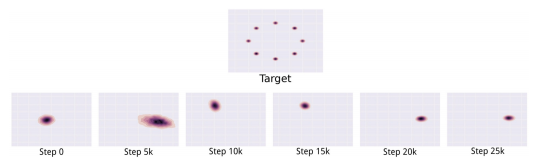
\includegraphics[width=9in]{../images/Unstable1}}

\slidetwo{Pros and Cons of GAN Evaluation Measures}{Borji, Oct 2018}

We would like a rate-distortion metric on distribution models.

\vfill
This has not yet been achieved for GANs.

\vfill
Evaluation of GANs always involves, at least in part, subjective judgments of naturalness.

\vfill
Sometimes automated metrics are also used.

\vfill
The above paper discusses various proposed automated metrics of GAN performance.  Current automated metrics are questionable.

\slide{}
\vfill
\centerline{\bf Contrastive GANS (TZ)}
\vfill\vfill

\slide{The Discriminator also Models the Population}

Fix the generator at a ``noise distribution'' $Q$ where $Q(y)$ is computable, and train a discriminator.

\vfill
{\color{red} $$\Psi^* = \argmin_\Psi E_{(i,y) \sim (\pop \uplus Q)}\;-\ln P_\Psi(i|y)$$}

\slide{The Discriminator also Models the Population}

{\color{red} $$\Phi^* = \argmin_\Phi E_{(i,y) \sim (\pop \uplus Q)}\;-\ln P_\Phi(i|y)$$}

Assuming Universality
$$P_{\Phi^*}(1|y) = P(1|y) = \frac{P(1\;\mathrm{and}\; y)}{P(y)} = \frac{\frac{1}{2}\mathrm{Pop}(y)}{\frac{1}{2}\mathrm{Pop}(y) + \frac{1}{2}Q(y)}$$

\vfill
$$P_{\Phi^*}(1|y)(\pop(y) + Q(y)) = \pop(y)$$

\vfill
{\color{red} $$ \frac{\pop(y)}{Q(y)} = \frac{P_{\Phi^*}(1|y)}{1-P_{\Phi^*}(1|y)}$$}

\slide{Discrimination}

The discrimination estimate of the population distribution is poor when the discrimination problem is easy --- when the discrimination loss can be driven close to zero.

\slidetwo{Noise Contrastive Estimation}{Gutmann and Hyv\"{a}rinen, 2010}

Consider a population distribution $\pop$ and a fixed generating distribution $Q$ where $Q(y)$ is computable.

\vfill
Define the distribution {\color{red} $\pop\hookrightarrow Q^k$} to be the result of drawing one ``positive'' from $\pop$ and $k$ IID negatives from $Q$;
then inserting the positive at a random position among the negatives; and returning $(i,y_1,\ldots,y_{k+1})$ where
$i$ is the index of the positive.

{\color{red} $$\Psi^* = \argmin_\Psi\; E_{(i,y_1,\ldots,y_{k+1})\sim (\pop\hookrightarrow Q^k)} \;- \ln P_\Psi(i|y_1,\ldots,y_{k+1})$$}

\slide{Contrastive Estimation}

{\color{red} $$\Psi^* = \argmin_\Psi\; E_{(i,y_1,\ldots,y_{k+1})\sim (\pop\hookrightarrow Q^k)} \;- \ln P_\Psi(i|y_1,\ldots,y_{k+1})$$}

\vfill
Note that $\pop\hookrightarrow Q^1$ requires a choice between two $y$'s while $\pop\uplus Q$ classifies a single $y$ --- these are different.

\vfill
The contrastive task gets more difficult as $k$ gets larger.


\slide{Constrastive Estimation}

$$\Psi^* = \argmin_\Psi E_{(i,y_1,\ldots,y_{k+1}) \sim (\pop\hookrightarrow Q^k)} \;- \ln P_\Psi(i|y_1,\ldots,y_{k+1})$$
{\color{red} $$P_\Psi(i|y_1,\ldots,y_{k+1}) \doteq \softmax_i s_\Psi(y_i)$$}

\vfill
{\color{red} Theorem}: Assuming universality:
\begin{eqnarray*}
s_{\Psi^*}(y) & = & \left(\ln \frac{\pop(y)}{Q(y)}\right) + C \;\;\;\mbox{for arbitrary $C$}\\
\\
{\color{red} \pop(y)} & {\color{red} =} & {\color{red} \softmax_y\;\;\; s_{\Psi^*}(y) - \ln Q(y)}\;\;\mbox{$Z$ must be estimated}
\end{eqnarray*}


\slide{Proof}
{\huge
\begin{eqnarray*}
{\color{red} P(i \;\mathrm{and}\;y_1,\ldots,y_{k+1})} & = & \frac{1}{k+1}\;\pop(y_i)\prod_{j \not = i}Q(y_j) \\
\\
& = & \alpha \frac{\pop(y_i)}{Q(y_i)},\;\;\;\alpha = \frac{1}{k+1} \prod_i Q(y_i) \\
\\
\\
{\color{red} P(i\;|\;y_1,\ldots y_{k+1})} & = & \frac{P(i\;\mbox{and} \; y_1,\ldots,y_{k+})}{\sum_i \;P(i \;\mbox{and}\; y_1,\ldots,y_{k+})} \\
\\
\\
& = & {\color{red} \softmax_i\; \left(\ln \frac{\pop(y_i)}{Q(y_i)}\right) + C}
\end{eqnarray*}
}

\slide{Constrastive Estimation}

Like the discrimination estimate, the contrastive estimate of $\pop$ is poor when the contrastive task is easy --- when the contrastive loss can be driven near zero.

\vfill
However, the contrastive task can be made more difficult by increasing $k$.

\slide{Contrastive GANs (TZ)}

Discriminative GAN:
{\color{red} $$\Phi^* = \argmax_\Phi \min_\Psi \;E_{(i,y) \sim (\pop \uplus P_\Phi)} - \ln P_\Psi(i|y)$$}

\vfill
Contrastive GAN:
{\color{red} $$\Phi^* = \argmax_\Phi \min_\Psi \;E_{(i,y_1,\ldots,y_{k+1}) \sim (\pop \hookrightarrow P_\Phi^k)} - \ln P_\Psi(i|y_1,\ldots,y_{k+1})$$}

\vfill
Assuming Universality:
{\color{red} $$P_{\Phi^*} = \pop$$}

\slide{Summary}

GANs have not generally proved useful for representation learning for discriminative tasks
such as image segmentation, speech recognition, or machine translation.

\vfill
I predict that there will ultimately be better ways to model distributions (as in language modeling).

\vfill
I predict that in a few years discriminators will be limited to enforcing perceptual naturalness in applications such as
text to speech and image decompression.

\slide{END}

}
\end{document}
